%  !TeX  root  =  user_guide.tex
\chapter{Trabalhando com dados OGC}\label{working_with_ogc}

% when the revision of a section has been finalized, 
% comment out the following line:
%\updatedisclaimer

QGIS suporta formatos WMS e WFS como base de dados. O suporte é nativo; WFS está implementado como um complemento.

\section{O que é um dado OGC?}\index{OGC!introduction}

A Open Geospatial Consortium (OGC), é uma organização internacional que possui mais de 300 organizações comerciais, governamentais e sem fins lucrativos espalhados ao redor do mundo. Seus membros desenvolvem e implementam padrões de conteúdo e de serviços geoespaciais, intercâmbio e processamento de dados geoespaciais.

Descrever uma base de dados modelo com características geográficas, pois é cada vez mais frequente a necessidade de atender especificações necessidades específicas de localização e de tecnologias geoespaciais interoperáveis, incluindo SIG. Maiores informações podem ser acessadas em \url{http://www.opengeospatial.org/}.

Importantes especificações de OGC:

\begin{itemize}
\item \textbf{WMS} - Web Map Service
\item \textbf{WFS} - Web Feature Service
\item \textbf{WCS} - Web Coverage Service
\item \textbf{CAT} - Web Catalog Service
\item \textbf{SFS} - Simple Features for SQL
\item \textbf{GML} - Geography Markup Language
\end{itemize}

Serviços OGC estão sendo largamente utilizados para troca de dados entre diferentes tipos de SIG e base de dados. O QGIS, até o presente momento, manipula apenas três das especificações acima, a SFS (com o suporte do provedor de dados PostgreSQL / PostGIS, ver seção \ref{label_postgis}), WFS e WMS como clientes.

\section{Cliente WMS}\label{sec:ogc-wms}\index{WMS!client}\index{OGC!WMS!client}\index{rasters!WMS}

\subsection{Visão geral do suporte WMS}\label{sec:ogc-wms-about}\index{WMS!client!about}

O QGIS atualmente funciona com um cliente WMS compreendendo servidores WMS 1.1, 1.1.1 e 1.3. Este cliente vem sendo testado em servidores de acesso público como DEMIS e JPL OnEarth.

Servidores WMS atendem a pedidos de clientes (e.g. QGIS) para mapas raster com uma dada extensão, conjunto de camadas, estilos de símbolos e transparência. O servidor WMS consulta suas bases locais, rasteriza o mapa, e envia-os para o cliente em um formato raster, geralmente em JPEG ou PNG.

O WMS é de forma genérica um serviço REST (Representational State Transfer) ao invés de um inflado serviço da web. Como tal, você pode realmente tomar as URLs geradas pelo
QGIS e utilizá-las em um navegador da Web para obter as mesmas imagens que o QGIS utiliza internamente. Isto pode ser útil para a solução de problemas, uma vez que existem
vários servidores WMS no mercado, e todos eles têm suas próprias
interpretações da norma WMS.
	
Camadas WMS  podem ser adicionadas, pura e simplesmente, desde que você saiba a URL para acessar o servidor WMS, você tenha uma ligação operacional com o servidor, e
compreenda o servidor HTTP como o mecanismo de transporte de dados.

\subsection{Selecionando Servidores WMS}\label{sec:ogc-wms-servers}\index{WMS!remote server!selection}

Não haverão servidores definidos na primeira utilização do recurso WMS. Você poderá iniciar um clicando o botão  \toolbtntwo{mActionAddWmsLayer}{Adicionar camada WMS} presente na barra de ferramentas, ou através do menu \mainmenuopt{Camada}>\dropmenuopttwo{mActionAddWmsLayer}{Adicionar camada WMS...}

O diálogo \dialog{Adicionar camada(s) de um servidor} para adicionar camadas de um servidor WMS. Oportunamente você poderá adicionar alguns servidores para rodar clicando em \button{Adicionar servidores padrão}. Isto irá adicionar os últimos três servidores para você usar, incluindo o servidor WMS da NASA (JPL). Para definir um novo serviço de servidor WMS na seção \tab{Conexões de servidores}, 
selecione \button{Novo}. Então, entre nos parâmetros para conectar ao servidor WMS desejado, como listado na tabela \ref{tab:wms_connection_parms}:

\begin{table}[ht]\index{WMS!client!connection parameters}
\centering
 \begin{tabular}{|l|p{5in}|}
\hline Nome & Um nome para esta conexão. Este nome será usado na caixa "Conexão de servidores" para distinguir de outras conexões com servidores WMS. \\
\hline URL \index{WMS!URL} & URL do servidor que provê o dado. Isto deve ser um destino acessível; o mesmo formato que seria usado para abrir uma conexão telnet ou pingar um destino. \\
\hline Senha & Senha para uma autenticação básica no servidor WMS. Este parâmetro é opcional.\\
\hline
\end{tabular}
\caption{Parâmetros de conexão WMS}\label{tab:wms_connection_parms}
\end{table}

Se você precisar especificar um servidor proxy para estar apto a receber serviços WMS da internet, você pode adicionar seu servidor proxy nas opções.
Escolha o menu \mainmenuopt{Configurações}  \arrow \dropmenuopttwo{mActionOptions}{Opções} e clique na aba \tab{Rede \& Proxy}. Nela você poderá adicionar as configurações proxy e habilitá-las acionando  \checkbox{Usar proxy de acesso a internet}.

Uma vez criada a uma nova conexão para um servidor WMS, ela será mantida para futuras seções do QGIS.

\begin{Tip}[ht]\caption{\textsc{Em URLs de servidores WMS}}
Esteja certo, quando entrar na URL de um servidor WMS, que você tem a URL base. Por exemplo, você não deveria ter fragmentos como \usertext{request=GetCapabilities} ou \usertext{versão=1.0.0}na sua URL.\index{WMS!remote server!URL}
\end{Tip}

\subsection{Carregar camadas WMS}\label{sec:ogc-wms-layers}\index{WMS!client!layers}

Uma vez preenchidos os parâmetros você poderá pressionar o botão
\button{Conectar} para resgatar as capacidades do servidor selecionado. Isto inclui imagens, camadas, estilos de camadas e projeções. Ao estabelecer a conexão, a velocidade de resposta dependerá da qualidade da conexão com o servidor WMS. Logo que iniciado o download de dados do servidor WMS, o processo poderá ser visualizado no canto inferior esquerdo da janela de diálogo do complemento WMS.

Sua tela irá mostrar algo como a Figura \ref{fig:connection_wms}, que mostra a resposta provida pelo servidor WMS JPL OnEarth WMS da NASA.

\minisec{Codificação de Imagem}

A seção \tab{Codificação de imagem} agora lista formatos que são suportados tanto pelo cliente, quanto pelo servidor. Escolha dependendo das suas necessidades de precisão.

\begin{Tip}[ht]\caption{\textsc{Codificação de Imagem}}
Você tipicamente espera que o servidor WMS te ofereça a escolha de compressão para os formatos JPEG ou PNG. O formato JPEG perde resolução na compressão, ao passo que o formato PNG reproduz com fidelidade o dado raster.

Use JPEG se você espera trabalhar com um dado WMS com menor resolução. Esta escolha reduz em 5 vezes o pedido de transferência comparado com PNG.

Use PNG se você precisa de representações mais fiéis do dado original, sabendo que para isso será necessário maior capacidade de transferência de dados. 
\index{WMS!image encoding}
\end{Tip}

\begin{figure}[ht]
\centering
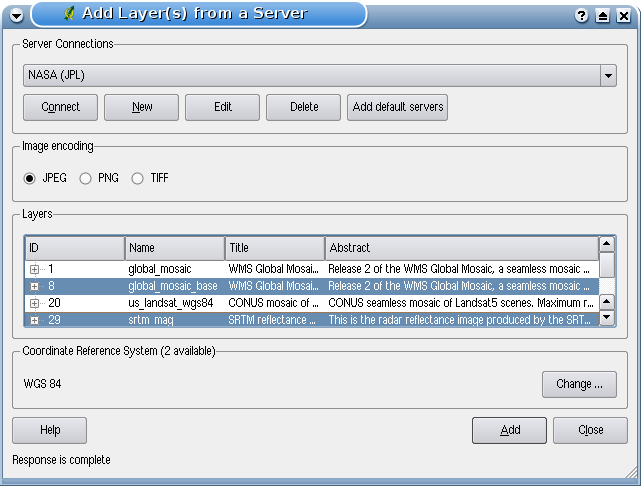
\includegraphics[clip=true,width=0.8\textwidth]{connection_wms}
\caption{Caixa de diálogo para adicionar um servidor WMS, mostrando as camadas disponíveis \nixcaption}\label{fig:connection_wms}
\end{figure}

\minisec{Opções}

A seção\tab{Options} fornece um campo de texto onde você pode adicionar um nome para a camada WMS. Este nome será apresentado na legenda depois de carregar a camada.

Se a OnlineRessource-URL a partir da GetCapabilities-document é diferente daquela URL inserida nos parâmetros de conexão, o QGIS perguntará a você qual URL deverá ser usada. Dependendo da sua resposta o QGIS marcará as caixas de opção baseada na sua resposta. Isso também pode ser ajustado com um \checkbox{Ignore GetMap URL} marcação e uma \checkbox{Ignore GetFeatureInfo URL} marcação separadamente, também depois de acionada.

\minisec{Camadas} \label{ogc-wms-layers}

A seção \tab{Camadas} lista as camadas disponíveis no servidor WMS. Você pode ver que algumas camadas são expansíveis, isto significa que as camadas podem ser mostradas com escolha de estilos de imagem.

Você pode selecionar muitas camadas de uma vez, mas um estilo de imagem por camada. Quando muitas camadas são selecionadas elas serão combinadas e transmitidas para o QGIS em uma vez.

\begin{Tip}[ht]\caption{\textsc{Ordenando camadas WMS}}
Nesta versão do QGIS, camadas WMS oferecidas por um servidor são sobrepostas na ordem listada na seção Camadas, de cima para baixo da lista.
Se você precisar sobrepor na ordem oposta, você pode selecionar a aba \tab{Ordem das Camadas}.
\index{WMS!remote server!layer ordering}
\end{Tip}

\minisec{Transparência}\label{ogc-wms-transparency}

Nesta versão do QGIS, a opção transparência é habilitada para estar sempre ligada, onde disponível.

\begin{Tip}[ht]\caption{\textsc{Transparência em camada WMS}}
A disponibilidade de transparência em imagens WMS depende do formato de imagem usado: PNG e GIF suportam transparência, JPEG não.
\index{WMS!layer transparency}
\end{Tip}

\minisec{Sistema de referência de coordenadas}
\index{WMS!CRS}
\index{WMS!coordinate reference system}
\index{OGC!CRS}
\index{OGC!coordinate reference system}
\index{Projections!WMS}
\index{Projections!CRS}
\index{Projections!coordinate reference system}
\index{CRS}
\index{coordinate reference system}
\index{SRS}
\index{Projections!SRS}

Um sistema de referência de coordenadas (SRC) é a terminologia OGC para uma projeção do QGIS.

Cada camada WMS pode ser apresentada em múltiplos SRCs, dependendo da capacidade do servidor WMS. Você pode observar que as \textsl{x} mudanças no \textsl{Sistema de referência de coordenada (x disponível)} conforme você seleciona ou desceleciona camadas na seção \tab{Camadas}.

Para escolher uma SRC, selecione \button{Mudar...} e uma tela similar a Figura \ref{fig:projections} na Seção \ref{label_projstart} aparecerá.
A principal diferença com a versão WMS da tela é que apenas aquelas SRCs suportadas pelo servidor WMS serão mostradas.

\begin{Tip}[ht]\caption{\textsc{Projeções WMS}}
Para obter melhores resultados, torne a camada WMS a primeira adicionada ao seu projeto. Isto permite a projeção do projeto herdar a SRC usada para reconhecer a camada WMS. Projeção On-the-fly (ver seção  \ref{sec:projection-specifying}) pode também ser usada para acessar qualquer camada vetorial subsequente a projeção do projeto. Nesta versão do QGIS, se você adicionar uma camada WMS mais tarde, e lhe atribuir uma SRC diferente da do projeto atual, resultados inesperados podem ocorrer.
\end{Tip}

% 
% server-search tab.
%
\subsection{Buscador de Servidores}
\label{sec:serversearch}
\index{WMS!serversearch}
\index{WMS!search}
\index{OGC!search}

No QGIS você pode buscar por servidores WMS. A Figura \ref{fig:searchtab} mostra a recentemente criada aba-\tab{buscar} com o Diálogo \dialog{Adicionar Camada(s) de um Servidor}.

\begin{figure}[ht]
  \centering
  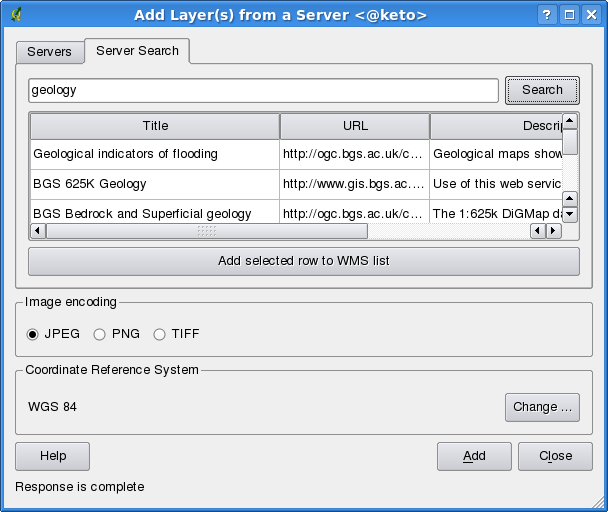
\includegraphics[clip=true,width=0.8\textwidth]{wms_server-search}
  	\caption{Diálogo para buscar servidores WMS através de algumas palavras-chave \nixcaption}\label{fig:searchtab}
\end{figure}

Como você pode perceber é possível entrar com uma palavra-chave no campo de texto e clicar no botão \button{Buscar}.

Após os resultados serão mostrados na aba abaixo do campo de texto.

Buscar na lista de resultados e observe a tabela. Para visualizar os resultados, selecione uma entrada da tabela, pressione o botão \button{Adicionar linha selecionada a lista WMS} e alterne pra a aba \tab{servidor}.

O QGIS atualizará automaticamente sua lista de servidores e o resultado da busca selecionado estará habilitado na lista de servidores WMS salvos.

Você precisa apenas solicitar a lista de camadas clicando no botão \button{Conectar}.

Esta opção é muito conveniente quando você precisa encontrar mapas através de palavras-chave específicas.

Esta opção é basicamente uma interface para a API de \url{http://geopole.org}.

%
% Tilesets
%
\subsection{Tilesets}\label{sec:tilesets}
\index{WMS!tileset}
\index{WMS!WMS-C}

Quando usar WMS-C (WMS armazenado) serviços como \url{http://labs.metacarta.com/wms-c/Basic.py} você estará apto a procurar através da aba \tab{tiles}-aba fornecida pelo servidor. Informação adicional como tilesize, formatos e SRCs suportados são listados nesta tabela.

Em combinação com esta feição você pode usar a escala tile deslizante a partir de  \mainmenuopt{Ver} \arrow \dropmenuopt{tile escala deslizante}, que fornece a você as escalas disponíveis a partir do servidor 'tile' com bom controle deslizante acoplado.

%
% Identify
%
\subsection{Usando a Ferramenta de Identificação}\label{sec:ogc-wms-identify}
\index{WMS!identify}
\index{identify!WMS}
\index{WMS!GetFeatureInfo}

Uma vez adicionado um servidor WMS, e se alguma camada do servidor WMS for consultável, você poderá usar a ferramenta \toolbtntwo{mActionIdentify}{Identificar} para selecionar um pixel do mapa que está na tela. A consulta é feita ao servidor a cada seleção efetuada.

Os resultados da consulta retornarão em modo texto. A formatação deste texto dependerá do tipo de servidor WMS usado.

% FIXME: GetFeatureInfo-Requests are done here?

\subsubsection{Propriedades de visualização}\label{sec:ogc-wms-properties}\index{WMS!properties}
\index{rasters!properties}

Uma vez adicionado o servidor WMS, você pode ver suas propriedades clicando com o botão direito na legenda, e selecionando \button{Propriedades}.


\minisec{Metadata Tab}\label{sec:ogc-wms-properties-metadata}
\index{rasters!metadata}
\index{WMS!metadata}
\index{WMS!capabilites}

A aba \tab{Metadata} mostra a abundância de informações sobre o servidor WMS, geralmente coletadas da declaração de capacidades retornadas daquele servidor.

Muitas definições podem ser colhidas lendo os padrões WMS \cite{OGCWMS010101web}, \cite{OGCWMS010300web}, abaixo seguem algumas definições mais comuns:

\begin{itemize}
\item \textbf{Propriedades do servidor}

\begin{itemize}
\item \textbf{Versão do WMS} - A versão suportada pelo servidor.

\item \textbf{Formatos de imagem} - A lista de tipos MIME que podem ser desenhadas no mapa. O QGIS suporta muitos tipos de formatos, sendo as mais frequentes \texttt{imagem/png} 
                                  e \texttt{imagem/jpeg}.

\item \textbf{Formatos de identidade} - A lista de tipos MIME que o servidor responde quando você usa a ferramenta de Identidade. Atualmente o QGIS suporta o tipo \texttt{text-plain}.

\end{itemize}

\item \textbf{Propriedades da camada}

\begin{itemize}
\item \textbf{Selecionada} - Se a camada está selecionada quando seu servidor foi adicionado ao projeto.

\item \textbf{Visível} - Se a camada está selecionada como visível na legenda. (Ainda não implementado nessa versão do QGIS).

\item \textbf{Identificável} - Se a camada permite ou não identificação de objetos quando a ferramenta Identificação é selecionada.

\item \textbf{Transparência} - Se a camada permite ou não ser renderizada com transparência. Esta versão do QGIS sempre usará transparência se esta for \textsl{Sim} e se o formato de imagem permita transparência.

% BM: doesn't seem to work?
%                                    (see Section
%                                    \ref{ogc-wms-transparency}
%                                    ).

\item \textbf{Aproximável} - Se a camada pode ser visualizada com aproximação pelo servidor. Esta versão do QGIS assume que todos as camadas WMS podem ser reunidas para \textsl{Sim}. Camadas deficientes podem retornar resultados ruins.

\item \textbf{Cascade Count}    - WMS servers can act as a proxy to other WMS servers to get
                                  the raster data for a layer.  This entry shows how
                                  many times the request for this layer is forwarded to peer
                                  WMS servers for a result.

\item \textbf{Largura fixa}, \textbf{Altura fixa}
                              - Se a camada possui ou não tamanho fixo de pixel. Esta versão do QGIS assume que todos as camadas WMS podem ser reunidas para não.
                                
\item \textbf{Caixa de limite em WGS 84} - Os limites da caixa da camada, em coordenadas WGS 84. Alguns servidores WMS não ajustam isto corretamente.(e.g. Coordenadas UTM será usada em substituição).  Se este é o casa, então a visão inicial da camada poderá ser desenhada com uma aparência "distante" pelo QGIS. O webmaster do WMS pode ser informado deste erro, no qual ele pode saber pelo caso podem ser  elementos WMS XML \texttt{LatLonBoundingBox}, \texttt{EX\_GeographicBoundingBox} ou o SRC:84 \texttt{BoundingBox}.

\item \textbf{Disponível no SRC} - As projeções que esta camada pode ser desenhada pelo servidor WMS. Estas estão listadas no formato WMS-nativo.

\item \textbf{Disponível no estilo} - Os estilos de imagem que esta camada pode ser desenhada no servidor WMS.

\end{itemize}

\end{itemize}


\subsection{Limitações do Cliente WMS}\label{sec:ogc-wms-limits}\index{WMS!client!limits}

Nem todas as possibilidades funcionais do cliente WMS foram incluídas nesta versão do QGIS. Algumas das mais notáveis exceções seguem abaixo:

\minisec{Editar Configurações da Camada WMS}
\index{WMS!layer settings!editing}

Uma vez que você completou o procedimento \toolbtntwo{mActionAddWmsLayer}{Adicionar camada WMS}, não haverá como mudar as configurações.

Uma forma de contornar isso é excluir a camada e iniciar novamente.

\minisec{Servidores WMS Solicitando Autenticação}
\index{WMS!remote server!authentication}
\index{WMS!remote server!basic authentification}

Apenas servidores públicos estão acessíveis.
Não há como aplicar uma combinação de nome de usuário e senha como uma autenticação ao servidor WMS. Você pode adicionar credenciais (opcional) quando adicionar um servidor WMS. Veja seção \ref{sec:ogc-wms-servers} para detalhes.

\begin{Tip}[ht]\caption{\textsc{Acessar Camadas-OGC Seguras}}
Se você precisar acessar camadas seguras, você pode usar InteProxy como um proxy de transporte, que suporte diversos métodos de autenticação. Mais informações podem ser encontradas no manual do InteProxy no website \url{http://inteproxy.wald.intevation.org}.
\index{WMS!secured layers!}\index{OGC!Authentication}
\end{Tip}

%
% WMS-server
%

\section{Servidor WMS}\label{sec:ogc-wmsserver}
\index{WMS!server}

O QGIS Mapserver é um implemento WMS 1.3 com código aberto que adiciona características avançadas de cartografia para mapeamento temático. O QGIS mapserver é uma aplicação FastCGI/CGI (Common Gateway Interface) escrita em C++ que trabalha junto com um servidor wwe (e.g. Apache, Lighttpd).

Ele usa o QGIS com backend para a lógica SIG e para a renderização de mapas. Além disso, a biblioteca Qt é usada para gráficos e para programação C++ em plataformas independentes. Em comparação com outros softwares WMS, o QGIS mapserver usa regras cartográficas em SLD/SE como uma linguagem de configuração, ambas para a configuração do servidor e para as regras cartográficas definidas pelo usuário.

Além disso, o projeto QGIS mapserver fornece o complemento "Publicar na Web", um complemento para o QGIS Desktop que exporta a camada atual e simbologia como um projeto da web para QGIS mapserver (contendo regras de visualização cartográfica expressas em SLD).

Como o QGIS desktop e o QGIS mapserver usam as mesmas bibliotecas de visualização, os mapas são publicados na web com a mesma cara do QGIS Desktop. O complemento Publicar na Web suporta atualmente simbolização básica, com regras de visualizações cartográficas mais complexas introduzidas manualmente. Como a configuração é realizada com o padrão SLD e possui extensões documentadas, há apenas uma linguagem padronizada para aprender, que simplifica a complexidade de criar mapas para a Web.

Maiores informações estão disponíveis em: \\
\url{http://karlinapp.ethz.ch/qgis\_wms/} \\
\url{http://www.qgis.org/wiki/QGIS\_mapserver\_tutorial} \\
\url{http://linfiniti.com/2010/08/qgis-mapserver-a-wms-server-for-the-masses/}



%
% WFS-client
%
\section{Cliente WFS e WFS-T}\label{sec:ogc-wfs}
\index{WFS!WFS-T}
\index{WFS!Transactional}

No QGIS, uma camada WFS se comporta como qualquer outra camada vetorial. Você pode identificar e selecionar feições e ver atributos de tabela. Uma exceção é que editar não é possível ainda. Para iniciar o plpugin WFS você precisa abrir \mainmenuopt{complementos} > 
\dropmenuopttwo{mActionShowPluginManager}{Gerenciador de complementos \dots}, ativar o 
\checkbox{complemento WFS} marcar e clicar \button{OK}. 

Um novo ícone \toolbtntwo{mIconAddWfsLayer}{Adicionar Camada WFS} aparecerá depois do ícone WMS. Clique nele para abrir o diálogo. Em Geral adicionar uma camada WFS é muito similar ao procedimento usado no WMS. A diferença está que não existem servidores definidos, assim, você precisará adicioná-los.

\subsection{Carregar uma camada WFS}

Como um exemplo nós utilizamos o servidor WFS DM solutions e mostramos uma camada. A URL é:
\begin{verbatim}
http://www2.dmsolutions.ca/cgi-bin/mswfs_gmap
\end{verbatim}

\begin{enumerate}
  \item Tenha certeza que o complemento WFS está carregado; se não estiver, abra o Gerenciador de Complementos e carregue-o
  \item Clique na ferramenta  
  \toolbtntwo{mIconAddWfsLayer}{Adicionar Camada WFS} 
  da barra de complementos
  \item Clique em \button{Novo} 
  \item Entre \inputtext{Nome}{DM Solutions} como o nome
  \item Entre com a URL (veja a página anterior)
  \item Clique \button{OK} 
  \item Escolha \selectstring{Conexões de Servidor}{DM Solutions} da caixa
  \item Clique \button{Conectar} 
  \item Espere pela lista de camadas aparecerem
  \item Clique na camada \clicklistitem{Parks}
  \item Clique \button{Ok} para adicionar a camada ao mapa
  \item Espere pacientemente pelo aparecimento das feições
\end{enumerate}

Note que o complemento WFS também reconhece as configurações do proxy que você fixar nas suas preferências.

\begin{figure}[ht]
  \centering
  	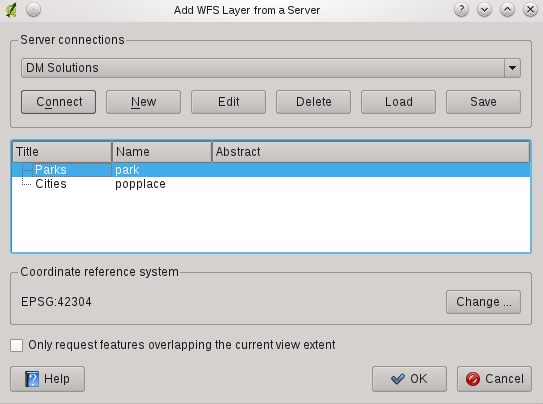
\includegraphics[clip=true,width=0.8\textwidth]{connection_wfs}
  	\caption{Adicionar uma camada WFS \nixcaption}\label{fig:wfs_dmsolutions}
\end{figure}

Sem usar a caixa de seleção \checkbox{Apenas o pedido de feições sobrepostas a visão atual extensão} o QGIS busca todas feições a partir do servidor WFS. Se você deseja apenas  uma pequena seleção baseada na sua extensão, aproxime para a área de interesse, solicite a camada WFS novamente e tenha certeza que você marcou a caixa de seleção acima. Basicamente, isto adiciona o parâmetro BBOX com os valores a partir da extensão atual à pesquisa WFS. Isto é extremamente útil quando você deseja apenas pedir \textbf{algumas} feições a partir de um grande conjunto de dados WFS.

Você poderá verificar o progresso do download no canto inferior esquerdo da janela principal do QGIS. 
Uma vez carregado a camada, você pode identificar e selecionar uma província ou duas e ver o atributo de tabela.

Lembre que este complemento trabalha bem com servidores MapServer WFS. Poderá ocorrer , que você experimente trocas de comportamento e paus. Você pode esperar aperfeiçoamentos em versões futuras deste complemento.

Isto significa que apenas WFS 1.0.0 é suportado. Até o momento não existem testes contrário a versões WFS mais recentes implementadas em outros servidores WFS. Se você encontrar problemas com quaisquer outros servidores WFS, por favor não exite em contatar a equipe de desenvolvimento. Por favor refira-se a Seção \ref{label_helpsupport} para maiores informações sobre as listas de e-mail.

\begin{Tip}[ht]\caption{\textsc{Procurar servidores WMS e WFS}}
Você pode adicionalmente procurar servidores WMS e WFS usando buscadores como Google ou outros. Existe uma lista de URLs públicas, algumas mantidas, outras não.
\index{WFS!remote server!}
\end{Tip} 

\begin{Tip}[ht]\caption{\textsc{Acessando Servidores WFS Seguros}}
Dentro do diálogo \dialog{Criar uma nova conexão WFS} descreve acidentalmente que o QGIS ainda não suporta conexões WFS autenticadas. Esperamos nas próximas versões atender também o suporte a servidores WFS autenticados. Enquanto isso você pode usar o InteProxy(\url{http://inteproxy.wald.intevation.org}) para acessar servidores WFS autenticados.
\index{WFS!authenticate remote server!}
\index{WFS!secured WFS server!}
\end{Tip} 

